%
%===============>>  ПРОБНИК 1 <<=============
%

%BEGIN_FOLD % ====>>_____ Вариант 1 _____<<====
\begin{training}[1]
	\title{Часть 1}
	\begin{listofex}
		%1
		\item Для объектов, указанных в таблице, определите, какими цифрами они обозначены на схеме. Заполните таблицу, в ответ запишите последовательность четырёх цифр.
			\begin{center}
			\footnotesize
			\begin{tabular}{|g|c|c|c|c|}
				\hline
				\textbf{Объекты}&Туалет&Детская&Гостиная&Кухня\\
				\hline
				\textbf{Цифры}&&&&\\
				\hline
			\end{tabular}
		\end{center}
			На плане изображена схема квартиры (сторона каждой клетки на схеме равна \( 1 \) м). Вход и выход осуществляются через единственную дверь.
		\gapwidth
		\begin{center}
			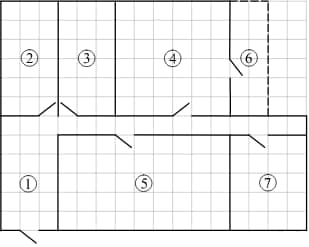
\includegraphics[align=t, width=0.5\linewidth]{\picpath/prob_2.2_1}
		\end{center}
		%2
		\item Краска продаётся в банках по \( 3 \) л. Сколько банок краски требуется купить, чтобы покрасить потолок в гостиной?
			\foranswer
		%3
		\item Найдите площадь, которую занимают детская и балкон. Ответ дайте в квадратных метрах.
		\foranswer
		%4
		\item Найдите расстояние между противоположными углами детской комнаты в метрах. Ответ запишите в виде \( \dfrac{d}{\sqrt{2}} \).
	\end{listofex}
	\newpage
	\phantom{Часть 1}
	\begin{listofex}[resume]
		%5
		\item 
			Хозяин квартиры планирует установить в квартире счётчик. Он рассматривает два варианта: однотарифный или двухтарифный счётчики. Цены на оборудование и стоимость его установки, данные о потребляемой мощности, и тарифах оплаты даны в таблице.
			Обдумав оба варианта, хозяин решил установить двухтарифный электросчётчик. Через сколько дней непрерывного использования электричества экономия от использования двухтарифного счётчика вместо однотарифного компенсирует разность в стоимости установки двухтарифного счётчика и однотарифного?
			\foranswer
		\gapwidth
		\begin{center}
			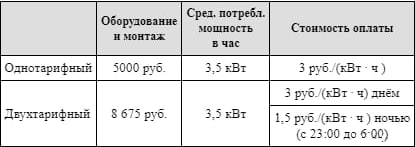
\includegraphics[align=t, width=0.8\linewidth]{\picpath/prob_2.2_2}
		\end{center}
		%6
		\item Найдите значение выражения: \( 2,5\cdot3,5-0,35 \)
		\foranswer
		%7
		\item Известно, что \( a<0<1 \). Выберите наименьшее из чисел. В ответе укажите номер правильного ответа.
		\begin{tasks}(1)
			\task \( a^2 \)
			\task \( a^3 \)
			\task \( -a \)
			\task \( \dfrac{1}{a} \)
		\end{tasks}
		\foranswer
		%8
		\item Найдите значение выражения \( \sqrt{7\cdot3^4}\cdot\sqrt{7\cdot2^2} \).
		\foranswer
		%9
		\item Решите уравнение \( (x+2)^2+(x-3)^2=2x^2 \)
		\foranswer
		\hphantom{Часть 1}
		%10
		\item .
		\foranswer
		%11
		\item .
		\foranswer
		%12
		\item .
		\foranswer
		%13
		\item .
		\foranswer
		%14
		\item .
		\foranswer
		%15
		\item .
		\foranswer
		%16
		\item .
		\foranswer
		%17
		\item .
		\foranswer
		%18
		\item .
		\foranswer
		%19
		\item .
		\foranswer
		\title{Часть 2}
		%20
		\item .
		%21
		\item .
		%22
		\item .
		%23
		\item .
		%24
		\item .
		%25
		\item .
	\end{listofex}
\end{training}
%END_FOLD

%BEGIN_FOLD % ====>>_____ Вариант 2 _____<<====
\begin{training}[2]
	\title{Часть 1}
	\begin{listofex}
		%1
		\item
		Длина зонта в сложенном виде равна \( 27 \) см и складывается из длины ручки (рис. \( 3 \)) и трети длины спицы (зонт в три сложения). Найдите длину спицы, если длина ручки зонта равна \( 6,8 \) см.\\\\
		Две подруги Оля и Аня задумались о том, как рассчитать площадь поверхности зонта.\\
		На первый взгляд зонт кажется круглым, а его купол напоминает часть сферы (сферический сегмент). Но если присмотреться, то видно, что купол зонта состоит из двенадцати отдельных клиньев, натянутых на каркас из двенадцати спиц (рис. \( 1 \)). Сферическая форма в раскрытом состоянии достигается за счёт гибкости спиц и эластичности ткани, из которой изготовлен зонт.\\
		Оля и Аня сумели измерить расстояние между концами соседних спиц \( a \). Оно оказалось равно \( 28 \) см. Высота купола зонта \( h \) (рис. \( 2 \)) оказалась равна \( 27 \) см, а расстояние \( d \) между концами спиц, образующих дугу окружности, проходящей через вершину зонта, --- ровно \( 108 \) см.
			\foranswer
		\gapwidth
		\begin{center}
			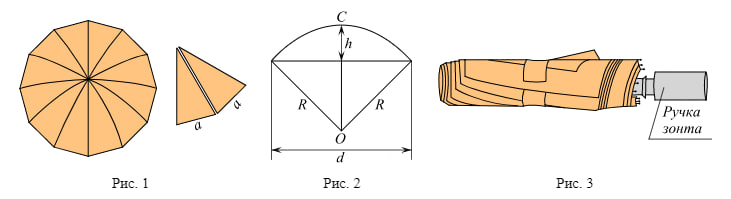
\includegraphics[align=t, width=\linewidth]{\picpath/prob_2.2_3}
		\end{center}
		\foranswer
		%2
		\item
		Поскольку зонт сшит из треугольников, рассуждала Оля, площадь его поверхности можно найти как сумму площадей треугольников. Вычислите площадь поверхности зонта методом Оли, если высота каждого равнобедренного треугольника, проведённая к основанию, равна \( 59 \) см. Ответ дайте в квадратных сантиметрах с округлением до десятков.
		\foranswer
		
		\newpage
		\hphantom{Часть 1}
		%3
		\item Аня предположила, что купол зонта имеет форму сферического сегмента. Вычислите радиус \( R \) сферы купола, зная, что \( OC=R \) (рис. \( 2 \)). Ответ дайте в сантиметрах.
		\foranswer
		%4
		\item Аня нашла площадь купола зонта как площадь поверхности сферического сегмента по формуле \( S=2\pi Rh \), где \( R \) --- радиус сферы, a \( h \) --- высота сегмента. Рассчитайте площадь поверхности купола способом Ани. Число \( \pi \)  округлите до \( 3,14 \). Ответ дайте в квадратных сантиметрах с округлением до целого.
		\foranswer
		%5
		\item Рулон ткани имеет длину \( 20 \) м и ширину \( 90 \) см. На фабрике из этого рулона были вырезаны треугольные клинья для \( 15 \) зонтов, таких же, как зонт, который был у Оли и Ани. Каждый треугольник с учётом припуска на швы имеет площадь \( 850 \) кв. см. Оставшаяся ткань пошла в обрезки. Сколько процентов ткани рулона пошло в обрезки?
		\foranswer
		%6
		\item Найдите значение выражения: \( \dfrac{11}{4,4\cdot2,5} \).
		\foranswer
		%7
		\item Какое из данных чисел принадлежит промежутку \( [7;8] \)? В ответ укажите номер правильного варианта.
		\begin{tasks}(1)
			\task \( \sqrt{7} \)
			\task \( \sqrt{8} \)
			\task \( \sqrt{48} \)
			\task \( \sqrt{56} \)
		\end{tasks}
		\foranswer
		%8
		\item Найдите значение выражения \( (4+\sqrt{5})^2+(4-\sqrt{5})^2 \)
		\foranswer
		\newpage
		\hphantom{Часть 1}
		%9
		\item Решите систему уравнений: \( \left\{
		\begin{array}{l}
			3x-y=-1,\\
			-x+2y=7
		\end{array}
		\right. \) В ответ запишите \( x+y \).
		\foranswer
		%10
		\item .
		\foranswer
		%11
		\item .
		\foranswer
		%12
		\item .
		\foranswer
		%13
		\item .
		\foranswer
		%14
		\item .
		\foranswer
		%15
		\item .
		\foranswer
		%16
		\item .
		\foranswer
		%17
		\item .
		\foranswer
		%18
		\item .
		\foranswer
		%19
		\item .
		\foranswer
		\title{Часть 2}
		%20
		\item .
		%21
		\item .
		%22
		\item .
		%23
		\item .
		%24
		\item .
		%25
		\item .
	\end{listofex}
\end{training}
%END_FOLD